\documentclass[tikz,border=10pt]{standalone}
\usepackage{ctex}
\usepackage{tikz}
\usepackage{slashed}
\usepackage{tikz-feynman}
\usepackage{amsmath}
\usetikzlibrary{positioning}
\usetikzlibrary{graphs}
\begin{document}

    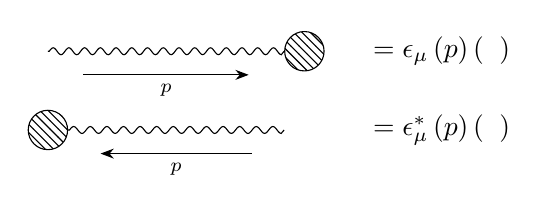
\begin{tikzpicture}[baseline]
        \begin{feynman}[small]
            %% fig a
            \vertex (a1) at (0,0);
            \vertex[right =3cm  of a1,blob] (a5){};
            % 对各个顶点连线
            \diagram*{
            { [edge=photon]
            (a1) --[momentum'={\scriptsize \(p\)}]  (a5),
            },
            };
            \node at (5,0) {$= \epsilon_\mu\left(p\right) \left(\text{入射}\right)$};
        \end{feynman}
        \begin{feynman}[small,yshift=-1cm]
            %% fig a
            \vertex [blob](a1) at (0,0) {};
            \vertex[right =3cm  of a1] (a5);
            % 对各个顶点连线
            \diagram*{
            { [edge=photon]
            (a1) --[reversed momentum'={\scriptsize \(p\)}]  (a5),
            },
            };
            \node at (5,0){$=\epsilon_{\mu}^{*}\left(p\right) \left(\text{出射}\right)$};
        \end{feynman}
        \end{tikzpicture} 

\end{document}
